% !TeX root = ../main.tex
% Add the above to each chapter to make compiling the PDF easier in some editors.

\chapter{Review of Literature and Research}\label{chapter:review_of_research}

\section{Types of Recommender Systems}
[kopi peyst]
Item recommendation approaches can be divided in two broad categories: per- sonalized and non-personalized. Among the personalized approaches are content- based and collaborative filtering methods, as well as hybrid techniques combining these two types of methods. The general principle of content-based (or cognitive) methods [4, 8, 42, 54] is to identify the common characteristics of items that have received a favorable rating from a user, and then recommend to this user new items that share these characteristics. Recommender systems based purely on content generally suffer from the problems of limited content analysis and over- specialization [63]. Limited content analysis occurs when the system has a limited amount of information on its users or the content of its items. For instance, privacy issues might refrain a user from providing personal information, or the precise content of items may be difficult or costly to obtain for some types of items, such as music or images. Another problem is that the content of an item is often insufficient to determine its quality. Over-specialization, on the other hand, is a side effect of the way in which content-based systems recommend new items, where the predicted rating of a user for an item is high if this item is similar to the ones liked by this user. For example, in a movie recommendation application, the system may recommend to a user a movie of the same genre or having the same actors as movies already seen by this user. Because of this, the system may fail to recommend items that are different but still interesting to the user.

Instead of depending on content information, collaborative (or social) filtering approaches use the rating information of other users and items in the system. The key idea is that the rating of a target user for a new item is likely to be similar to that of another user, if both users have rated other items in a similar way. Likewise, the target user is likely to rate two items in a similar fashion, if other users have given similar ratings to these two items. Collaborative approaches overcome some of the limitations of content-based ones. For instance, items for which the content is not available or difficult to obtain can still be recommended to users through the feedback of other users. Furthermore, collaborative recommendations are based on the quality of items as evaluated by peers, instead of relying on content that may be a bad indicator of quality. Finally, unlike content-based systems, collaborative filtering ones can recommend items with very different content, as long as other users have already shown interest for these different items.

Collaborative filtering approaches can be grouped in the two general classes of neighborhood and model-based methods. In neighborhood-based (memory-based [10] or heuristic-based [2]) collaborative filtering [14, 15, 27, 39, 44, 48, 57, 59, 63], the user-item ratings stored in the system are directly used to predict ratings for new items. This can be done in two ways known as user-based or item-based recommendation. User-based systems, such as GroupLens [39], Bellcore video [27], and Ringo [63], evaluate the interest of a target user for an item using the ratings for this item by other users, called neighbors, that have similar rating patterns. The neighbors of the target user are typically the users whose ratings are most correlated to the target user’s ratings. Item-based approaches [15, 44, 59], on the other hand, predict the rating of a user for an item based on the ratings of the user for similar items. In such approaches, two items are similar if several users of the system have rated these items in a similar fashion.

In contrast to neighborhood-based systems, which use the stored ratings directly in the prediction, model-based approaches use these ratings to learn a predictive model. Salient characteristics of users and items are captured by a set of model parameters, which are learned from training data and later used to predict new ratings. Model-based approaches for the task of recommending items are numerous and include Bayesian Clustering [10], Latent Semantic Analysis [28], Latent Dirich- let Allocation [9], Maximum Entropy [72], Boltzmann Machines [58], Support Vector Machines [23], and Singular Value Decomposition [6, 40, 53, 68, 69]. A survey of state-of-the-art model-based methods can be found in Chap. 3 of this book.

Finally, to overcome certain limitations of content-based and collaborative filtering methods, hybrid recommendation approaches combine characteristics of both types of methods. Content-based and collaborative filtering methods can be combined in various ways, for instance, by merging their individual predictions into a single, more robust prediction [8, 55], or by adding content information into a collaborative filtering model [1, 3, 51, 65, 71]. Several studies have shown hybrid recommendation approaches to provide more accurate recommendations than pure content-based or collaborative methods, especially when few ratings are available [2].

\section{Neighborhood-Based Approach}

\subsection{Introduction}
[kopi peyst]
While recent investigations show state-of-the-art model-based approaches superior to neighborhood ones in the task of predicting ratings [40, 67], there is also an emerging understanding that good prediction accuracy alone does not guarantee users an effective and satisfying experience.

Model-based approaches excel at characterizing the preferences of a user with latent factors. For example, in a movie recommender system, such methods may determine that a given user is a fan of movies that are both funny and romantic, without having to actually define the notions “funny” and “romantic”. This system would be able to recommend to the user a romantic comedy that may not have been known to this user. However, it may be difficult for this system to recommend a movie that does not quite fit this high-level genre, for instance, a funny parody of horror movies. Neighborhood approaches, on the other hand, capture local associations in the data. Consequently, it is possible for a movie recommender system based on this type of approach to recommend the user a movie very different from his usual taste or a movie that is not well known (e.g. repertoire film), if one of his closest neighbors has given it a strong rating. This recommendation may not be a guaranteed success, as would be a romantic comedy, but it may help the user discover a whole new genre or a new favorite actor/director. -> Model based suck at serendipity

\begin{itemize}
	\item Simplicity: Neighborhood-based methods are intuitive and relatively simple to implement. In their simplest form, only one parameter (the number of neighbors used in the prediction) requires tuning.
	\item  Justifiability: Such methods also provide a concise and intuitive justification for the computed predictions. For example, in item-based recommendation, the list of neighbor items, as well as the ratings given by the user to these items, can be presented to the user as a justification for the recommendation. This can help the user better understand the recommendation and its relevance, and could serve as basis for an interactive system where users can select the neighbors for which a greater importance should be given in the recommendation [6].
	\item Efficiency: One of the strong points of neighborhood-based systems are their efficiency. Unlike most model-based systems, they require no costly training phases, which need to be carried at frequent intervals in large commercial applications. These systems may require pre-computing nearest neighbors in an offline step, which is typically much cheaper than model training, providing near instantaneous recommendations. Moreover, storing these nearest neighbors requires very little memory, making such approaches scalable to applications having millions of users and items.
	\item Stability: Another useful property of recommender systems based on this approach is that they are little affected by the constant addition of users, items and ratings, which are typically observed in large commercial applications. For instance, once item similarities have been computed, an item-based system can readily make recommendations to new users, without having to re-train the system. Moreover, once a few ratings have been entered for a new item, only the similarities between this item and the ones already in the system need to be computed.
\end{itemize}

While neighborhood-based methods have gained popularity due to these advan- tages, they are also known to suffer from the problem of limited coverage, which causes some items to be never recommended. Also, traditional methods of this category are known to be more sensitive to the sparseness of ratings and the cold-start problem, where the system has only a few ratings, or no rating at all, for new users and items. Section 2.5 presents more advanced neighborhood-based techniques that can overcome these problems.

\subsection{User-Based Rating Prediction}

[ Kitapta 2.3.1] 2 Sayfa kadar

\subsection{User-Based Classification}

[ Kitapta 2.3.2] 0.5 Sayfa kadar

\subsection{Regression vs Classification}

[kopi -peys, genel daha uzun bahsedilebilir ve belki resim eklenebilir]
The choice between implementing a neighborhood-based regression or classifica- tion method largely depends on the system’s rating scale. Thus, if the rating scale is continuous, e.g. ratings in the Jester joke recommender system [20] can take any value between -10 and 10, then a regression method is more appropriate. On the contrary, if the rating scale has only a few discrete values, e.g. “good” or “bad”, or if the values cannot be ordered in an obvious fashion, then a classification method might be preferable. Furthermore, since normalization tends to map ratings to a continuous scale, it may be harder to handle in a classification approach.
Another way to compare these two approaches is by considering the situation where all neighbors have the same similarity weight. As the number of neighbors used in the prediction increases, the rating rui predicted by the regression approach will tend toward the mean rating of item i. Suppose item i has only ratings at either end of the rating range, i.e. it is either loved or hated, then the regression approach will make the safe decision that the item’s worth is average. This is also justified from a statistical point of view since the expected rating (estimated in this case) is the one that minimizes the RMSE. On the other hand, the classification approach will predict the rating as the most frequent one given to i. This is more risky as the item will be labeled as either “good” or “bad”. However, as mentioned before, taking risks may be desirable if it leads to serendipitous recommendations.

\subsection{Item-Based Recommendation}

[ Kitapta 2.3.2] 1 Sayfa kadar

\subsection{Item-Based vs User-Based Recommendation}

[ Kitapta 2.3.3] 1 Sayfa kadar

\subsection{Steps of Neighborhood Methods}

three very important considerations in the implementation of a neighborhood-based recommender system are (1) the normalization of ratings, (2) the computation of the similarity weights, and (3) the selection of neighbors. This section reviews some of the most common approaches for these three components, describes the main advantages and disadvantages of using each one of them, and gives indications on how to implement them.

\subsubsection{Normalization of Ratings}
[2.4.1.1 ve 2.4.1.2' i de ekle]
In some cases, rating normalization can have undesirable effects. For instance, imagine the case of a user that gave only the highest ratings to the items he has purchased. Mean-centering would consider this user as “easy to please” and any rating below this highest rating (whether it is a positive or negative rating) would be considered as negative. However, it is possible that this user is in fact “hard to please” and carefully selects only items that he will like for sure. Furthermore, normalizing on a few ratings can produce unexpected results. For example, if a user has entered a single rating or a few identical ratings, his rating standard deviation will be 0, leading to undefined prediction values. Nevertheless, if the rating data is not overly sparse, normalizing ratings has been found to consistently improve the predictions [25, 29].

Comparing mean-centering with Z-score, as mentioned, the second one has the additional benefit of considering the variance in the ratings of individual users or items. This is particularly useful if the rating scale has a wide range of discrete values or if it is continuous. On the other hand, because the ratings are divided and multiplied by possibly very different standard deviation values, Z-score can be more sensitive than mean-centering and, more often, predict ratings that are outside the rating scale. Lastly, while an initial investigation found mean-centering and Z-score to give comparable results [25], a more recent one showed Z-score to have more significant benefits [29].

Finally, if rating normalization is not possible or does not improve the results, another possible approach to remove the problems caused by the rating scale variance is preference-based filtering. The particularity of this approach is that it focuses on predicting the relative preferences of users instead of absolute rating values. Since an item preferred to another one remains so regardless of the rating scale, predicting relative preferences removes the need to normalize the ratings. More information on this approach can be found in [12, 18, 32, 33].

\subsubsection{Computation of Similarity Weights}


The similarity weights play a double role in neighborhood-based recommendation methods: (1) they allow to select trusted neighbors whose ratings are used in the prediction, and (2) they provide the means to give more or less importance to these neighbors in the prediction. The computation of the similarity weights is one of the most critical aspects of building a neighborhood-based recommender system, as it can have a significant impact on both its accuracy and its performance.

[2.4.2.1, 2.4.2.2]  cosine vector, person correlation, adjusted cosine, mean squared prediction


There are also some considerations: [en iyisi bu kismi ayri chapter yapip bunu subsubsection yap]

Significance of weights: 1 paragraph
Variance of Ratings: 1 paragraph, mesela godfather'i herkes seviyor => IDF yap

\subsubsection{Neigborhood Selection}


The number of nearest-neighbors to select and the criteria used for this selection can also have a serious impact on the quality of the recommender system. The selection of the neighbors used in the recommendation of items is normally done in two steps: (1) a global filtering step where only the most likely candidates are kept, and (2) a per prediction step which chooses the best candidates for this prediction.

Prefiltering[aslinda subsubsec]: In large recommender systems that can have millions of users and items, it is usually not possible to store the (non-zero) similarities between each pair of users or items, due to memory limitations. Moreover, doing so would be extremely wasteful as only the most significant of these values are used in the predictions. The pre- filtering of neighbors is an essential step that makes neighborhood-based approaches practicable by reducing the amount of similarity weights to store, and limiting the number of candidate neighbors to consider in the predictions. There are several ways in which this can be accomplished:

\begin{itemize}
	\item Top-n filtering: For each user or item, only a list of the N nearest-neighbors and their respective similarity weight is kept. To avoid problems with efficiency or accuracy, N should be chosen carefully. Thus, if N is too large, an excessive amount of memory will be required to store the neighborhood lists and predicting ratings will be slow. On the other hand, selecting a too small value for N may reduce the coverage of the recommendation method, which causes some items to be never recommended.
	\item Threshold filtering: Instead of keeping a fixed number of nearest-neighbors, this approach keeps all the neighbors whose similarity weight’s magnitude is greater than a given threshold wmin. While this is more flexible than the previous filtering technique, as only the most significant neighbors are kept, the right value of wmin may be difficult to determine.
	\item Negative filtering: In general, negative rating correlations are less reliable than positive ones. Intuitively, this is because strong positive correlation between two users is a good indicator of their belonging to a common group (e.g., teenagers, science-fiction fans, etc.). However, although negative correlation may indicate membership to different groups, it does not tell how different are these groups, or whether these groups are compatible for some other categories of items.
\end{itemize}

Actual Prediction[aslinda subsubsec]: Once a list of candidate neighbors has been computed for each user or item, the prediction of new ratings is normally made with the k-nearest-neighbors, that is, the k neighbors whose similarity weight has the greatest magnitude. The choice of k can also have a significant impact on the accuracy and performance of the system.

As shown in Table 2.3, the prediction accuracy observed for increasing values of k typically follows a concave function. Thus, when the number of neighbors is restricted by using a small k (e.g., k < 20), the prediction accuracy is normally low. As k increases, more neighbors contribute to the prediction and the variance introduced by individual neighbors is averaged out. As a result, the prediction accuracy improves. Finally, the accuracy usually drops when too many neighbors are used in the prediction (e.g., k > 50), due to the fact that the few strong local relations are “diluted” by the many weak ones. Although a number of neighbors between 20 to 50 is most often described in the literature, see e.g. [24, 26], the optimal value of k should be determined by cross-validation.

On a final note, more serendipitous recommendations may be obtained at the cost of a decrease in accuracy, by basing these recommendations on a few very similar users. For example, the system could find the user most similar to the active one and recommend the new item that has received the highest rated from this user.

\subsection{Conclusion}


One of the earliest approaches proposed for the task of item recommendation is neighborhood-based recommendation, which ranks among the most popular methods for this problem. Although quite simple to describe and implement, this recommendation approach has several important advantages, including its ability to explain a recommendation with the list of the neighbors used, its computational and space efficiency which allows it to scale to large recommender systems, and its marked stability in an online setting where new users and items are constantly added. Another of its strengths is its potential to make serendipitous recommendations that can lead users to the discovery of unexpected, yet very interesting items.

In the implementation of a neighborhood-based approach, one has to make several important decisions. Perhaps the one having the greatest impact on the accu- racy and efficiency of the recommender system is choosing between a user-based and an item-based neighborhood method. In typical commercial recommender systems, where the number of users far exceeds the number of available items, item-based approaches are typically preferred since they provide more accurate recommendations, while being more computationally efficient and requiring less frequent updates. On the other hand, user-based methods usually provide more original recommendations, which may lead users to a more satisfying experience. Moreover, the different components of a neighborhood-based method, which include the normalization of ratings, the computation of the similarity weights and the selection of the nearest-neighbors, can also have a significant influence on the quality of the recommender system. For each of these components, several different alternatives are available. Although the merit of each of these has been described in this document and in the literature, it is important to remember that the “best” approach may differ from one recommendation setting to the next. Thus, it is important to evaluate them on data collected from the actual system, and in light of the particular needs of the application.

Finally, when the performance of a neighborhood-based approach suffers from the problems of limited coverage and sparsity, one may explore techniques based on dimensionality reduction or graphs. Dimensionality reduction provides a compact representation of users and items that captures their most significant features. An advantage of such approach is that it allows to obtain meaningful relations between pairs of users or items, even though these users have rated different items, or these items were rated by different users. On the other hand, graph-based techniques exploit the transitive relations in the data. These techniques also avoid the problems of sparsity and limited coverage by evaluating the relationship between users or items that are not “directly connected”. However, unlike dimensionality reduction, graph-based methods also preserve some of the “local” relations in the data, which are useful in making serendipitous recommendations.

 \begin{figure}[!ht]
	\centering
	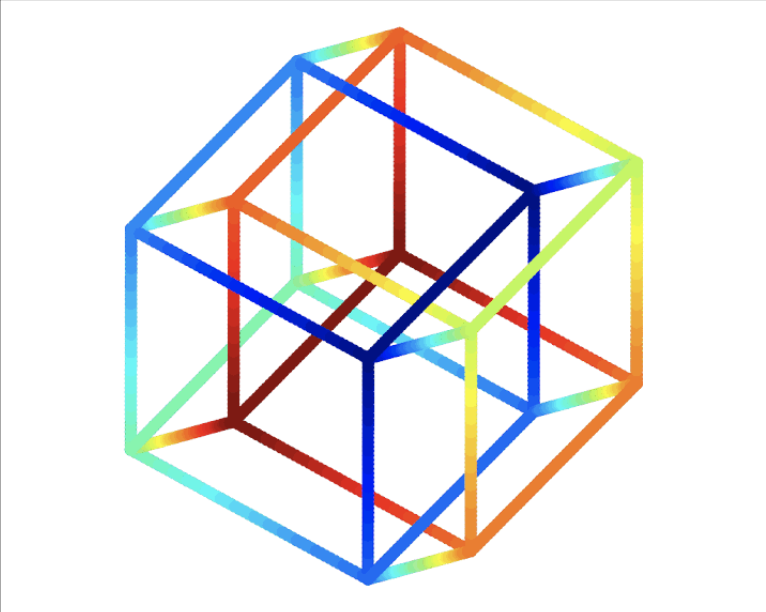
\includegraphics[width=0.75\textwidth]{figures/DimensionalityReduction.png}
	\caption{2D representation of a 4D cube. The colors indicate the depth in fourth dimension ~\parencite{lee2007nonlinear}.}
	\label{fig:embedding-projection-example}
\end{figure}


